\documentclass[10pt,a4paper]{article}
\usepackage[utf8]{inputenc}

\usepackage[landscape,margin=1cm]{geometry}
\usepackage[english]{babel}

\date{} % disables the default date
\title{How to Get your First Job in \textbf{Data Analytics}}
\author{Author: \href{https://www.linkedin.com/in/igorshkokov/}{Igor Shkokov}}
\usepackage[default]{raleway}
\usepackage{fontawesome}
\usepackage[T1]{fontenc}

\usepackage{minted}  
\usemintedstyle{default}  

\usepackage{hyperref}
\usepackage{enumitem}
\usepackage{lipsum}

\usepackage{xcolor}
\definecolor{customcolor}{HTML}{616AC5}
\definecolor{alert}{HTML}{CD5C5C}
\definecolor{w3schools}{HTML}{4CAF50}
\definecolor{subbox}{gray}{0.60}
\definecolor{codecolor}{HTML}{FFC300}
\colorlet{xx}{customcolor}


%--------------------------Editor mode.

\usepackage
[citestyle=authoryear,
sorting=nty,	  		%Sorts bibliography by year, name, title
autocite=footnote, 		%Autocite command generates footnotes
autolang=hyphen, 		
mincrossrefs=1, 	
backend=biber]
{biblatex}

\DeclareFieldFormat{postnote}{#1}
\DeclareFieldFormat{multipostnote}{#1}
\DeclareAutoCiteCommand{footnote}[f]{\footcite}{\footcites}

\bibliography{literature}
%----------------------------------------
%--------------------------------------------------------------------------------
\usepackage{tcolorbox}

\tcbuselibrary{most,listingsutf8,minted}

\tcbset{tcbox width=auto,left=1mm,top=1mm,bottom=1mm,
right=1mm,boxsep=1mm,middle=1pt}

\newenvironment{mycolorbox}[2]{%
\begin{tcolorbox}[grow to left by=-1em,grow to right by=-1em,capture=minipage,fonttitle=\large\bfseries, enhanced jigsaw,boxsep=1mm,colback=#1!30!white,on line,tcbox width=auto, toptitle=0mm,colframe=#1,opacityback=0.7,nobeforeafter,title=#2]%
}{\end{tcolorbox}\\[0.2em]}

\newenvironment{subbox}[2]{%
\begin{tcolorbox}[capture=minipage,fonttitle=\normalsize\bfseries, enhanced jigsaw,boxsep=1mm,colback=#1!30!white,on line,tcbox width=auto,left=0.3em,top=1mm, toptitle=0mm,colframe=#1,opacityback=0.7,nobeforeafter,title=#2]\footnotesize %
}{\normalsize\end{tcolorbox}\vspace{0.1em}}

\newenvironment{multibox}[1]{%
\begin{tcbraster}[raster columns=#1,raster equal height,nobeforeafter,raster column skip=1em,raster left skip=1em,raster right skip=1em]}{\end{tcbraster}}

\newenvironment{textbox}[1]{\begin{mycolorbox}{customcolor}{#1}}{\end{mycolorbox}}

%-------------------------------
\newtcblisting{codebox}[2]{colback=codecolor!5,colframe=codecolor!80!black,listing only, 
minted options={numbers=left,style=default,fontsize=\tiny,breaklines,autogobble,linenos,numbersep=3mm},
left=5mm,enhanced,
title=#2, fonttitle=\bfseries,
listing engine=minted,minted language=#1}

%--------------------------------------------------------------------------------
\newcommand{\punkti}{~\lbrack\dots\rbrack~}

\renewenvironment{quote}
               {\list{\faQuoteLeft\phantom{ }}{\rightmargin\leftmargin}%
                \item\relax\scriptsize\ignorespaces}
               {\unskip\unskip\phantom{xx}\faQuoteRight\endlist}
               

%--------------------------------------------------------------------------------
\newcommand{\bgupper}[3]{\colorbox{#1}{\color{#2}\huge\bfseries\MakeUppercase{#3}}}
\newcommand{\bg}[3]{\colorbox{#1}{\bfseries\color{#2}#3}}

\newcommand{\mycommand}[2]{{\ttfamily\detokenize{#1}}~\dotfill{}~{\footnotesize #2}\\}
\newcommand{\sep}{{\scriptsize~\faCircle{ }~}}


\newcommand{\bggreen}[1]{\medskip\bgupper{w3schools}{black}{#1}\\[0.5em]}
\newcommand{\green}[1]{\smallskip\bg{w3schools}{white}{#1}\\}
\newcommand{\red}[1]{\smallskip\bg{alert}{white}{#1}\\}

\usepackage{multicol}
\setlength{\columnsep}{30pt}

\setlength{\parindent}{0pt}
\pagestyle{empty}

\usepackage{csquotes}

\newcommand{\loremipsum}{Lorem ipsum dolor sit amet.}


\begin{document}
\small
\begin{multicols}{3}

\maketitle
\thispagestyle{empty}
\scriptsize

%-----------------------------------------------------
\begin{textbox}{Applying}
\emph{Everyone gets through this - and you will too.}
\begin{itemize}
  \item \textbf{Apply often} (10--20 roles/week)
  \item Tailor your CV for each application \textbf{(1 custom > 5 generic)}
  \item Use a job \href{https://huntr.co/product/job-tracker}{tracker}
  \item Most companies use \href{https://en.wikipedia.org/wiki/Applicant_tracking_system}{ATS}. Use \href{https://www.jobscan.co/}{Jobscan}
  \item \textbf{Reach out directly} to HR or team leads on LinkedIn
  \item Use an email \href{https://chromewebstore.google.com/detail/email-tracker/bnompdfnhdbgdaoanapncknhmckenfog}{tracker} to know if your email was read
  \item Set job \href{https://www.linkedin.com/jobs/jam/}{alerts}
  \item Don't stress about a perfect GitHub profile

\end{itemize}

\emph{99\% rejection rate is normal --- \textbf{always} ask for feedback.} 
\end{textbox}

%-----------------------------------------------------
\begin{textbox}{If You're Not Getting Interviews}

\emph{Key question: How is my application different from a 100 others?}

\begin{itemize}
    \item \textbf{Do Pet Projects}
    \item \href{https://www.linkedin.com/pulse/art-asking-referral-linkedin-comprehensive-guide-simon-siew-nz8ff/}{Look for referrals inside the company} 
    \item Highlight domain expertise, if you have it
    \item Ask friends in HR or Data to review your CV
    \item Use \href{https://www.tealhq.com/post/xyz-resume}{XYZ method} for your CV
    \item \href{https://adplist.org/}{\textbf{Get a mentor}}  

	\end{itemize}
\emph{Applied 100 times with no luck? Change your approach.}
\end{textbox}
%-----------------------------------------------------

\begin{textboxWhite}{}
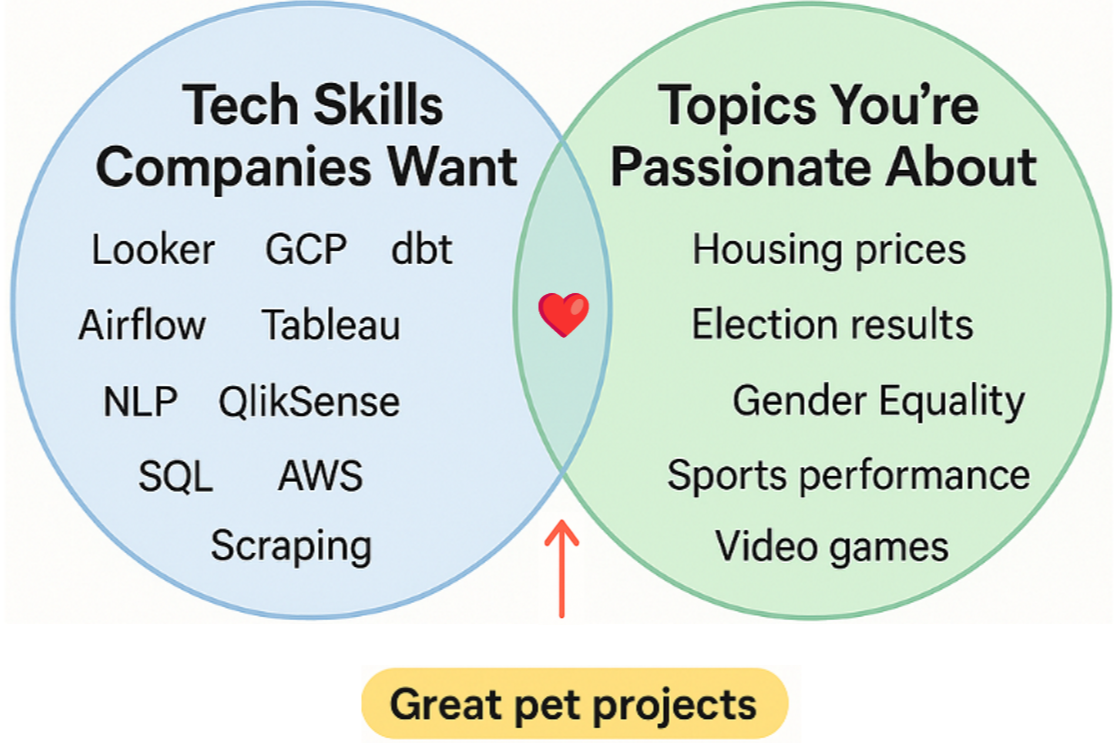
\includegraphics[width=\textwidth]{image.png}
\end{textboxWhite}

%-----------------------------------------------------
	
\begin{textbox}{Pet Projects}
\emph{I landed my first job in Data by sending \underline{\href{https://www.youtube.com/watch?v=54jvW1ulaP0&t=961s}{this}} with every application.}

\begin{itemize}
    \item Try to find \textbf{unexpected} insights
    \item Make it \textbf{shareable} and \textbf{presentable} (YouTube > all)
\end{itemize}

\textbf{Follow the process:}
\begin{itemize}
    \item Define a Question $\Rightarrow$ Data Acquisition $\Rightarrow$ Cleaning/Wrangling $\Rightarrow$ Analysis (SQL, Python) $\Rightarrow$ Visualization (BI) $\Rightarrow$ Insights/Recommendations
\end{itemize}
\textbf{Examples:}
\begin{itemize}
    \item \href{https://youtube.com/watch?v=HKuhMtrEgDE}{Paris Real Estate Pet Project on Youtube}
    \item \href{https://youtube.com/watch?v=HKuhMtrEgDE}{Video Game Project on YouTube} 
    \item \href{https://public.tableau.com/app/profile/ryansoares/viz/GoogleSearchTrendsMostSuccessfulSongsof2020/Dashboard}{2020 Songs Tableau Public dashboard} 
    \item \href{https://medium.com/@joseikwame/cyclistic-bike-share-analysis-case-study-99095c444505}{Bike Rental Project on Medium} 
    \item \href{https://github.com/amritachinnam/Customer-Data-Analytics-Power-BI}{Smart Pet Devices Analysis on GitHub}
\end{itemize}

\textit{Aim to simulate the tasks and the stack of the companies you’re applying to.}

\end{textbox}

%-----------------------------------------------------
\begin{textbox}{Hard Skills Focus Areas}
	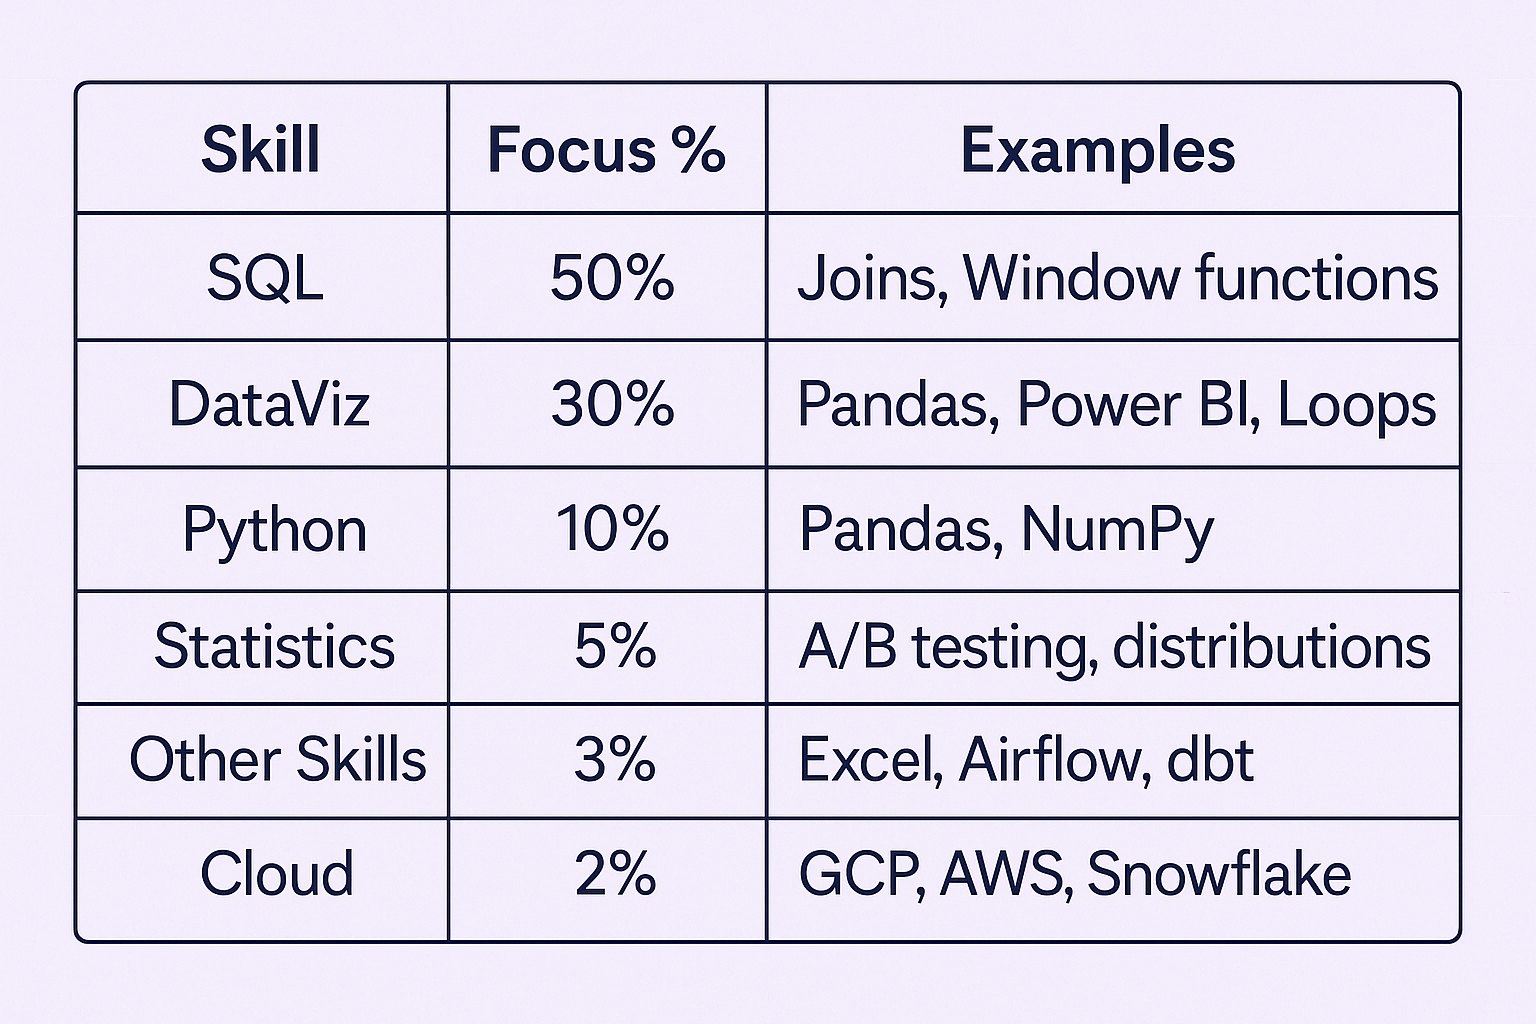
\includegraphics[width=\textwidth]{table2.png}
\end{textbox}

%-----------------------------------------------------
\begin{textbox}{If You Get an Interview}

\textit{Well done! Here are the usual steps — some of them may be skipped or reordered, but typically:}

\begin{itemize}
    \item HR call $\Rightarrow$ Technical test $\Rightarrow$ Presentation $\Rightarrow$ Another tech interview (live coding, etc) $\Rightarrow$ Team fit interview $\Rightarrow$ Offer
  \end{itemize}

On each step, \textbf{ask how many other candidates} are in the process. Remember, it’s a competition — \textbf{each step could be the final one.}
\begin{itemize}    
\item If you reach the technical test stage:
  \begin{itemize}
    \item  Dedicate as much time as possible to it
    \item \textbf{Always} go beyond than what’s required
    \item Look for \textbf{unexpected} insights 
    \item Include next steps
  \end{itemize}
  \item Smart questions are better than smart answers. Ask:
  \begin{itemize}
    \item \textit{“Who held this role before, and why did they leave?”}
    \item \textit{“What are the current data challenges your team is facing?”}
    \item \textit{“Isn’t [this tech in their stack] outdated? Have you considered [this new tech that’s more innovative]?”}
  \end{itemize}
\end{itemize}

\end{textbox}

%-----------------------------------------------------
\begin{textbox}{Courses and Practice}
\emph{Practice often, especially before a live coding test.}

\begin{itemize}
    \item SQL: \href{https://datalemur.com/}{\textbf{DataLemur}}, \href{https://www.sqlnoir.com/}{SQL Noir}, \href{https://mystery.knightlab.com/}{SQL Mystery}
    \item Python: \href{https://datacamp.com/}{\textbf{DataCamp}}
    \item Datasets: \href{https://www.kaggle.com/}{\textbf{Kaggle}}
    \item Coding challenges: \href{https://leetcode.com/}{Leetcode}, \href{https://www.stratascratch.com/}{Stratascratch}
\end{itemize}
\end{textbox}

%-----------------------------------------------------
\begin{textbox}{What to Read}
\textbf{Blogs:}
\begin{itemize}
    \item \href{https://towardsdatascience.com/}{Towards Data Science}
    \item \href{https://www.kdnuggets.com/}{Kdnuggets}
    \item \href{https://ourworldindata.org/}{Our World in Data}
    \item \href{https://www.voronoiapp.com/}{Voronoi}
    \item \href{https://reddit.com/r/dataanalysis/}{\texttt{r/dataanalysis}}
\end{itemize}
\textbf{Newsletters:} \href{https://tldr.tech/newsletters}{TLDR}, \href{https://flowingdata.com/newsletter/}{FlowingData}, \href{https://www.blef.fr/}{Blef.fr}, \href{https://www.holoniq.com/newsletters}{HolonIQ}

\textbf{Books:}
\begin{itemize}
    \item \href{https://www.amazon.com/Designing-Your-Life-Well-Lived-Joyful/dp/1101923083}{Designing Your Life} (Part 7: How Not to Get a Job)
    \item \href{https://www.amazon.com/Wishcraft-How-What-Really-Want/dp/0345465180}{Wishcraft: How to Get What Your Really Want}
\end{itemize}
\end{textbox}

%-----------------------------------------------------
\begin{textbox}{One Last Thought}
\emph{What would you do if you had unlimited money?}
\end{textbox}
%-----------------------------------------------------


\date{\today}
\end{multicols}
\end{document}
